\chapter{Results}\label{ch:results}

This chapter details the equilibrium and stability limits of hydrogen exsolution from
H$_2$--MgSiO$_3$ mixtures. We begin by characterizing the binodal and spinodal of the
published mixing model across pressure and composition, establishing the metastable window.
Building on this, we analyze the hydrogen inventory that delayed exsolution could withhold
along cooling paths. Subsequently, the published fit is audited against its source
simulations and recalibrated against the same data. The chapter concludes with a test of
whether coexistence data can identify the spinodal at all.

\section{Phase Boundaries and the Metastable Window}\label{sec:window}

Figure~\ref{fig:phase_maps} shows the binodal and spinodal temperatures of the published
model as a function of local hydrogen mass fraction at 2, 5 and 10\,GPa. The binodal is
flat-topped: its crest at 2\,GPa lies at $T_C = \pubTcTwo{}$\,K and $x_C = \pubXc{}$
($w = \pubWc{}$\,wt\%), and it falls only slowly away from $x_C$. The spinodal touches the
binodal at the critical point and falls steeply on the hydrogen-poor side. Spinodals exist
only above $w = \pubThreshold{}$\,wt\%. Below this threshold a parcel can still separate in
equilibrium, but its homogeneous state never becomes unstable, so separation always requires
nucleation (Appendix~\ref{app:thermo}).

\begin{figure}[t]
\centering
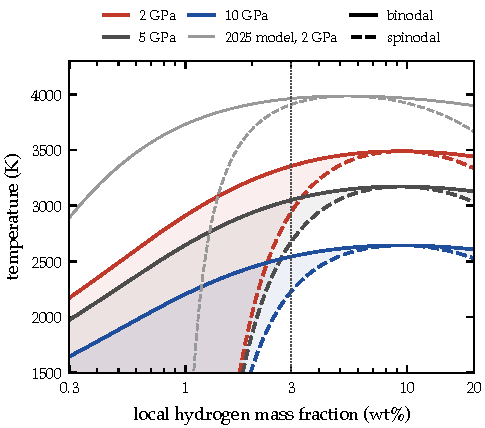
\includegraphics[width=\columnwidth]{fig3_1_phase_maps}
\thesiscaption{Binodal and spinodal temperatures of the published mixing model.}{Solid
lines show the binodal, dashed lines the spinodal, at 2, 5 and 10\,GPa; shading marks the
metastable window. Grey lines show the historical 2025 parameterization at 2\,GPa. The dotted
line marks the 3\,wt\% baseline.}
\label{fig:phase_maps}
\end{figure}

For the baseline parcel of 3\,wt\% hydrogen at 2\,GPa, the binodal lies at \pubTbTwo{}\,K and
the spinodal at \pubTspTwo{}\,K. The metastable interval is therefore \pubIntTwo{}\,K
(Table~\ref{tab:onsets}). It shrinks to \pubIntFive{}\,K at 5\,GPa and \pubIntTen{}\,K at
10\,GPa, because both onset temperatures scale with $1+P/\pi$. At 10\,GPa the spinodal lies
below the coldest two-phase simulation (2,500\,K), so it is an extrapolation.

\begin{table}[t]
\thesiscaption{Onset temperatures for a parcel with 3\,wt\% local hydrogen.}{$f_{\rm H}$ is
the fraction of hydrogen that equilibrium places in the H-rich phase at the spinodal.}
\label{tab:onsets}
\small\centering
\setlength{\tabcolsep}{4.5pt}
\begin{tabular}{@{}lrrrr@{}}
\toprule
Model, $P$ & $T_b$ (K) & $T_{\rm sp}$ (K) & $\Delta T_{\rm ms}$ (K) & $f_{\rm H}$ (\%)\\
\midrule
2026 fit, 2\,GPa & \pubTbTwo & \pubTspTwo & \pubIntTwo & \pubFhTwo\\
2026 fit, 5\,GPa & \pubTbFive & \pubTspFive & \pubIntFive & \pubFhFive\\
2026 fit, 10\,GPa & \pubTbTen & \pubTspTen & \pubIntTen & \pubFhTen\\
2025 fit, 2\,GPa & \oldTbTwo & \oldTspTwo & \oldIntTwo & \oldFhTwo\\
Wrong basis, 2\,GPa & \wrongTbTwo & \wrongTspTwo & \wrongIntTwo & \wrongFhTwo\\
\bottomrule
\end{tabular}
\end{table}

The composition basis matters. The historical 2025 parameterization gives an interval of only
\oldIntTwo{}\,K, and importing the 2026 parameters without the basis conversion gives
\wrongIntTwo{}\,K. With the correct conversion the interval is about nine times larger.
Changing $A$, $B$, $\tau$ and $|\pi|$ by $\pm10\%$ gives intervals of
\stressIntLo{}--\stressIntHi{}\,K. These stress cases are not calibrated uncertainties;
Section~\ref{sec:recalibrated} derives uncertainties from the data.

\section{Hydrogen Inventory along Cooling Paths}\label{sec:inventory}

Figure~\ref{fig:inventory}a follows the 3\,wt\% parcel as it cools. In the equilibrium limit
the H-rich phase appears at $T_b$ and grows on further cooling. In the delayed limit nothing
separates until $T_{\rm sp}$, where the parcel jumps to the equilibrium state. At the spinodal
the equilibrium limit already places \pubFhTwo{}\% of all hydrogen in the H-rich phase, while
the delayed limit still holds it in the homogeneous parcel.

\begin{figure}[t]
\centering
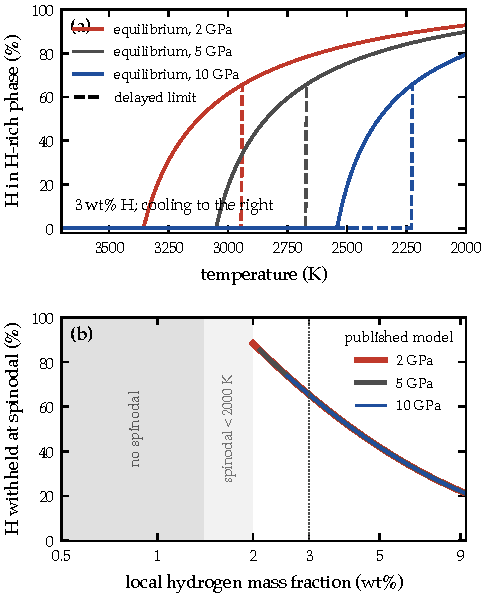
\includegraphics[width=\columnwidth]{fig3_2_inventory}
\thesiscaption{Hydrogen withheld by delayed exsolution.}{(a) Fraction of all hydrogen in
the H-rich phase for a 3\,wt\% parcel cooling at 2, 5 and 10\,GPa, in the equilibrium limit
(solid) and the delayed limit (dashed). (b) Fraction withheld at the spinodal as a function of
local hydrogen mass fraction. The curves for the three pressures coincide.}
\label{fig:inventory}
\end{figure}

At 3,000\,K and 2\,GPa the baseline parcel is metastable. Equilibrium would place
\eqFhThreeThousand{}\% of its hydrogen in the H-rich phase, which is \gramsWithheld{}\,g of the
30\,g of hydrogen in each kilogram of parcel, whereas the delayed limit has not separated at
all. Equilibration would lower the Gibbs energy by \energyLowering{}\,kJ per native mole. This
is a free-energy difference, not a prediction of released heat.

The withheld fraction at the spinodal is the same at 2, 5 and 10\,GPa to within
\fhPressureSpread{}, or \fhPressureSpreadAll{} within 0.1\,wt\% of the critical composition,
where the lever rule becomes ill-conditioned (Figure~\ref{fig:inventory}b). It falls from 88\%
at 2\,wt\%, the lowest composition whose spinodal lies above 2,000\,K, to about 21\% near the
critical composition. The pressure invariance
follows from the separable form of Eq.~(\ref{eq:gs26}) (Appendix~\ref{app:thermo}); it is not
independent evidence.

\section{Audit of the Published Fit against its Source Data}\label{sec:audit}

Our implementation reproduces the published model (Section~\ref{sec:verification}), so any
mismatch with the source simulations belongs to the published fit itself. The fit agrees with
all ten one-phase runs. For the two-phase run at 1.65\,GPa, its gap at 3,500\,K lies entirely
above the bulk composition of the cell, a miss of \pubMissOneSixFive{}\,K in temperature.
It reproduces both compositions within the quoted $\pm0.05$ for only one of the four
two-phase runs (Table~\ref{tab:ed1}, Figure~\ref{fig:audit}b).

\begin{figure*}[t]
\centering
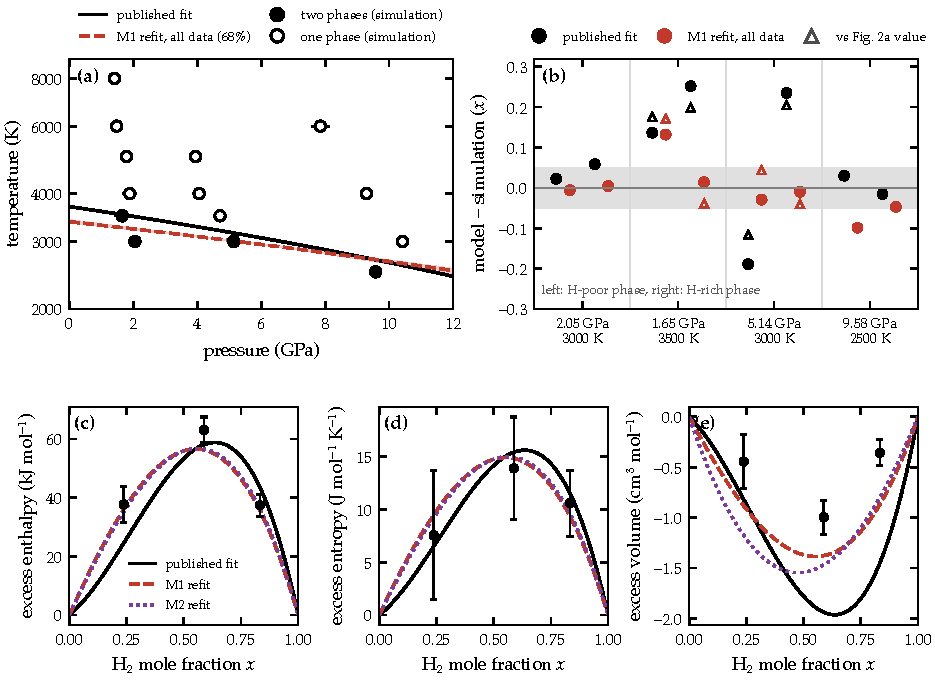
\includegraphics[width=\textwidth]{fig3_3_source_audit}
\thesiscaption{Audit of the published fit against its source simulations.}{(a) Phase state of
the 14 coexistence runs (filled: two phases; open: one phase) with the published critical
curve (black) and the critical curve of the refit to all data (red, 68\% band). (b) Model
minus simulation for the eight coexisting compositions, against ED Table~1 (circles) and the
digitized Figure~2a (triangles); the grey band is the quoted $\pm0.05$. (c--e) Excess
enthalpy, entropy and volume of the homogeneous simulations at 5\,GPa and 4,000\,K
(symbols, 1$\sigma$), with the published fit and the refits of classes M1 and M2.}
\label{fig:audit}
\end{figure*}

\paragraph{Near-critical runs.} The largest misses occur for the two runs closest to the
critical curve. The published $T_C$ lies \tcAboveRunNearCritLow{}\,K above the run at
1.65\,GPa and 3,500\,K, and \tcAboveRunNearCritHigh{}\,K above the run at 5.14\,GPa and
3,000\,K. For the first run the model predicts a gap centred at $x \approx 0.71$, whereas the
simulation shows a gap centred at 0.52. For exactly these two runs the source table and the
source figure disagree. The digitized Figure~2a places the pairs at
(\figLoOneSixFive{}, \figHiOneSixFive{}) and (\figLoFiveOneFour{}, \figHiFiveOneFour{}),
whereas ED Table~1 lists (0.458, 0.576) and (0.587, 0.706). The differences range from
\diffLoFiveOneFour{} to \diffHiOneSixFive{}. For the two wide-gap runs, table and figure agree
to within \digMarker{}.

In all four two-phase runs, the per-phase atom numbers in ED Table~1 add up to the full
simulation cell, so every interfacial atom is counted in one of the two phases. With sharp
interfaces this matters little. Near $T_C$, however, interfaces broaden, and such a count
pulls both compositions toward the bulk composition of the cell, which is 0.526 and 0.629 for
these runs. The two composition estimators described in the source methods
\cite{gilmore2026} could therefore differ most for exactly these runs, as observed. We treat
the near-critical compositions as uncertain at the 0.04--0.07 level. This is an inference from
the published numbers, not a demonstrated cause.

\paragraph{Homogeneous simulations.} The homogeneous simulations reveal a second mismatch
(Figure~\ref{fig:audit}c--e). The published fit predicts an excess volume of
$\vModMid$\,cm$^3$\,mol$^{-1}$ at $x = \xMid{}$, whereas the simulations give
$\vObsMid \pm \vSigMid$\,cm$^3$\,mol$^{-1}$. Because the excess volume sets the pressure dependence of $T_C$,
the value $\pi = -35$\,GPa reproduces the critical curve between 2 and 10\,GPa, but the
directly simulated volumes imply a pressure scale about twice as large in magnitude. The fit
also underestimates the excess enthalpy at $x = 0.24$. In total, the published fit has
$\chi^2 = \pubChiPhase{}$ for the 14 phase states, \pubChiComp{} for the eight compositions
and \pubChiHom{} for the nine homogeneous properties.

These comparisons reproduce checks against the data from which the fit was built. They are
not independent validation, and they do not show that any simulation is wrong. They show
that one four-parameter model cannot follow all of the source data at once.

\section{Recalibrated Delayed-Exsolution Interval}\label{sec:recalibrated}

Table~\ref{tab:recalibration} and Figure~\ref{fig:posteriors} summarize the nine refits.
Refitting the published form (class M1) to all data lowers $\chi^2$ from \pubChiTotal{} to
\ChiMOneTable{}. The best fit is much less asymmetric than the published one
(Table~\ref{tab:map}) and has a lower critical temperature,
$T_C(2\,{\rm GPa}) = \TcMOneTable{}$\,K (68\% range \TcMOneTableLo{}--\TcMOneTableHi{}\,K). It
pays for this with the phase state of the run at 1.65\,GPa and 3,500\,K, which it places
\MissMOneTable{}\,K above its binodal. The metastable interval of the baseline parcel shrinks
to \IntMOneTable{}\,K (\IntMOneTableLo{}--\IntMOneTableHi{}\,K), and the withheld fraction to
\FhMOneTable{}\%.

\begin{table*}[t]
\thesiscaption{Recalibration of the hydrogen--silicate mixing model.}{$\chi^2$ terms at the
best fit for the 14 phase states, the 8 compositions and the 9 homogeneous properties, and
posterior medians with 68\% ranges of the critical temperature at 2\,GPa, the metastable
interval and the withheld hydrogen fraction for a 3\,wt\% parcel at 2\,GPa. Fits marked
$\dagger$ leave out data (dashes), so their $\chi^2$ cannot be compared with the others.}
\label{tab:recalibration}
\small\centering
\begin{tabular}{@{}lrrrlll@{}}
\toprule
Fit & $\chi^2_{\rm phase}$ & $\chi^2_{\rm comp}$ & $\chi^2_{\rm hom}$ & $T_C$ (K) &
$\Delta T_{\rm ms}$ (K) & $f_{\rm H}$ (\%)\\
\midrule
\inputtable{tables/recalibration.tex}
\bottomrule
\end{tabular}
\end{table*}

\begin{figure*}[t]
\centering
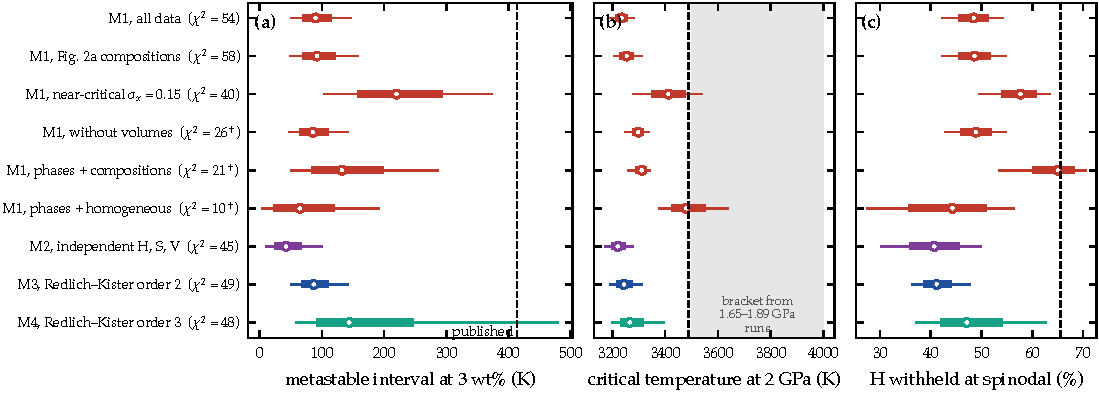
\includegraphics[width=\textwidth]{fig3_4_posteriors}
\thesiscaption{Posterior distributions of the delayed-exsolution quantities.}{(a) Metastable
interval, (b) critical temperature at 2\,GPa and (c) withheld hydrogen fraction for a 3\,wt\%
parcel at 2\,GPa, for each model class and data treatment. Thick bars show 68\% and thin bars
95\% intervals; open circles mark medians. Dashed lines mark the published fit; the grey band
in (b) is the bracket set by the two-phase run at 1.65\,GPa and the one-phase run at
1.89\,GPa, drawn without correction to 2\,GPa. Labels give the best-fit $\chi^2$; fits marked
$\dagger$ use fewer data.}
\label{fig:posteriors}
\end{figure*}

The data treatments show which data drive this shift (Table~\ref{tab:map}). Without the
homogeneous data, the fit returns to the published asymmetry, $B/A = \BAMOnePhaseComp{}$
against 5.65, but with interaction parameters three times larger and a lower $\tau$. Its
interval is \IntMOnePhaseComp{}\,K, not \pubIntTwo{}\,K, so the asymmetry alone does not set the
interval: the excess entropy and the strength of the interaction matter as much. With the
homogeneous data but without the compositions, the excess is nearly symmetric,
$B/A = \BAMOnePhaseHom{}$, and the interval is \IntMOnePhaseHom{}\,K. The compositions themselves
discriminate weakly between these fits: their misfit is $\chi^2_{\rm comp} =
\ChiCompMOnePhaseComp{}$ for the strongly and \ChiCompMOneTable{} for the weakly asymmetric
fit. The difference lies mainly in the phase states and the
homogeneous data. Using the Figure~2a compositions instead of ED Table~1 gives
\IntMOneFigure{}\,K, and dropping the excess volumes gives \IntMOneNoVolume{}\,K: the volume
mismatch controls the pressure dependence of $T_C$, but hardly the interval at 2\,GPa. Giving
the two near-critical runs a composition uncertainty of 0.15 raises the asymmetry to
$B/A = \BAMOneInflated{}$ and lengthens the interval to \IntMOneInflated{}\,K.

Every refit that uses the coexisting compositions places the run at 1.65\,GPa and 3,500\,K
between \missLo{} and \missHi{}\,K above its binodal. This reflects a tension within the source
data. The narrow gap at 5.14\,GPa and 3,000\,K requires $T_C$ close to 3,000\,K at that pressure,
whereas the two-phase state at 1.65\,GPa requires $T_C > 3{,}500$\,K. A linear critical curve
meets both only if it falls by more than about \slopeMinimum{}\,K per GPa. The published fit falls
by \slopePublished{}\,K per GPa, and the fit to phase states and homogeneous data by
\SlopeMOnePhaseHom{}\,K per GPa.

The more flexible classes fit the data with $\chi^2 = \ChiMTwo{}$ (M2), \ChiMThree{} (M3) and
\ChiMFour{} (M4), against \ChiMOneTable{} for M1. Their intervals are \IntMTwo{},
\IntMThree{} and \IntMFour{}\,K. None of the classes fits all data within the quoted errors: for 31 data
points, $\chi^2$ stays between \ChiMTwo{} and \ChiMOneTable{}. Across all nine refits the median
interval ranges from \IntRangeLo{} to \IntRangeHi{}\,K, compared with \pubIntTwo{}\,K for the
published fit (Table~\ref{tab:recalibration}, Figure~\ref{fig:posteriors}a). The most flexible class, M4, does not
exclude the published value: its 95\% range is \IntMFourLoNinetyFive{}--\IntMFourHiNinetyFive{}\,K. Every fit met our convergence criterion of a
split-chain $\hat R < 1.1$; the largest value is \maxRhat{}.

\begin{figure*}[t]
\centering
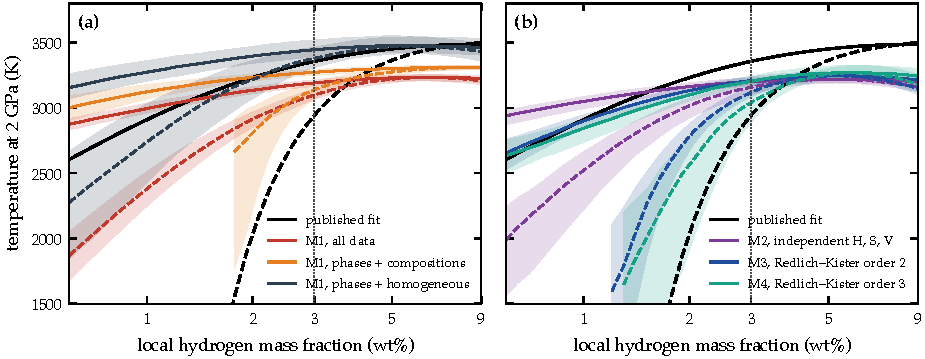
\includegraphics[width=\textwidth]{fig3_5_posterior_phase_diagrams}
\thesiscaption{Posterior binodals and spinodals at 2\,GPa.}{Medians (lines) and 68\% bands of
the binodal (solid) and spinodal (dashed) for (a) class M1 with three data treatments and (b)
classes M2--M4 with all data, compared with the published fit (black).}
\label{fig:posterior_diagrams}
\end{figure*}

\section{Identifiability of the Spinodal}\label{sec:identifiability}

The perturbation of Eq.~(\ref{eq:bump}) leaves the binodal, the equilibrium free energy and
every homogeneous state outside the gap unchanged; we verified this to within
$4\times10^{-12}$\,J\,mol$^{-1}$. It nevertheless moves the spinodal
(Figure~\ref{fig:identifiability}). At $\lambda = 8$ the 3\,wt\% spinodal rises by
\bumpThree{}\,K, the 5\,wt\% spinodal falls by \bumpFiveAbs{}\,K and the 2\,wt\% spinodal rises by
\bumpTwo{}\,K. Coexistence data alone therefore cannot identify the spinodal. Any spinodal
inferred from them is a property of the assumed functional form.

\begin{figure*}[t]
\centering
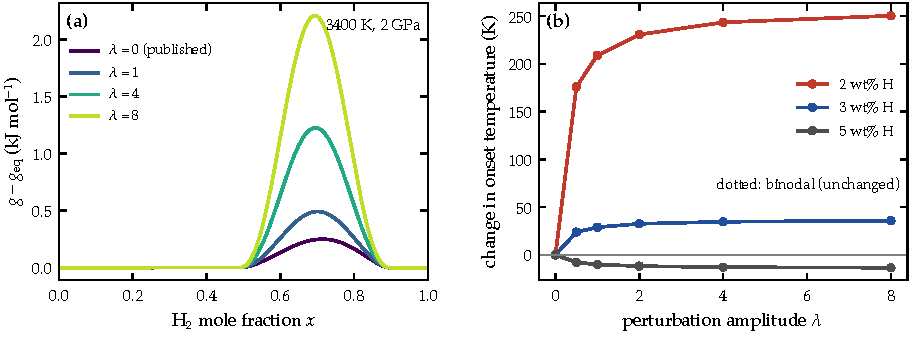
\includegraphics[width=\textwidth]{fig3_6_identifiability}
\thesiscaption{Two free energies with the same equilibrium but different spinodals.}{(a)
Homogeneous Gibbs energy above the equilibrium (convex-envelope) free energy at 3,400\,K and
2\,GPa for perturbation amplitudes $\lambda$ = 0 to 8. Outside the gap all curves are zero.
(b) Change of the spinodal (solid) and binodal (dotted) temperatures with $\lambda$ for 2, 3
and 5\,wt\% local hydrogen.}
\label{fig:identifiability}
\end{figure*}
